\documentclass[conf]{new-aiaa}
%\documentclass[journal]{new-aiaa} for journal papers
\usepackage[utf8]{inputenc}

\usepackage{graphicx}
\usepackage{amsmath}
\usepackage[version=4]{mhchem}
\usepackage{siunitx}
\usepackage{longtable,tabularx}
\setlength\LTleft{0pt} 
\captionsetup{justification=centering}
\title{Anatomy of Superconducting Qubits}

\author{Quantum Wizards: Josh, Ian, Mark, Sam, Daniil, Bassel, Joe, Javad}

\begin{document}
\today
\maketitle

\section{Introduction}
This book is meant to introduce a reader not familiar with quantum mechanics and computing to the principles of superconducting qubits. First we will discuss \textit{Elements of Quantum Computing} to review the history of quantum computing, looking at the discoveries made in the field. \cite{akama2015elements}

After a tour through the history of quantum computing we will introduce superconducting qubits, how they work in theory, and in practice.

We then introduce programming for qubits, algorithms that make use of quantum computers, and simulating physics on quantum computers.

\subsection{History of Quantum Computing}

\textit{Elements of Quantum Computing} by Seiki Akama is an introduction to quantum computing which does not require previous knowledge of computer science or quantum mechanics. It is a great reference to use to structure a discussion on the history of quantum computing. The first chapter outlines the history of quantum computers and quantum mechanics through brief descriptions of the works of various physicists who contributed to those fields.

Chapter 2 is an introduction to the computer. It discusses models of computers such as Neumann-type and Turing Machine. Here we are introduced to what a computer does and how they work through binary operations.

Chapter 3 is an introduction to quantum mechanics (QM). It talks about both wave mechanics and matrix mechanics. It will also introduce Dirac notation and interpretation of quantum mechanics. 

Chapter 4 combines the information from the previous chapters. It discusses quantum computers (QC) and how they are different from classical computers. Akama also talks about some interesting properties of QC, like the no-cloning theorem, as well as algorithms that take advantage of qubits.

Chapter 5 discusses applications of QC known when the book was published. Quantum communications, teleportation, and programming.

Chapter 6 forcasts future directions of QC and challenges that scientists face in developing QC.

%\section{Review}

\subsubsection{Introduction}

This section does an excellent job of summarizing the history of quantum computers (QC) and quantum mechanics (QM). The writing is effective at conveying the progress made by scientists in a brief and interesting way. The information is organised chronologically which makes it intuitive to see how discoveries followed from previous ones. The section on the history of QM where each scientist and their contribution to the field is accompanied with a picture of the physicist and a summary of their academic career is especially enjoyable.

The story starts in 1980 with Benioff who first proposed a quantum mechanical model of computers. \cite{benioff1980computer} In 1982 Feynman realised that a quantum computer would be well suited to simulate physics, compared to classical computers where computational time would make some problems intractable. \cite{feynman1982simulating} Deutsch also proposed a model for a quantum computer as well as a theory of a quantum gate in 1985 and 1988 respectively. \cite{deutsch1985quantum, deutsch1995universality} Generalizing Deutsch's model, Bernstein and Vazirani proposed a universal quantum turing machine in 1993 which also proves that classical turing machines and quantum turing machines have equivalent computational power. \cite{bernstein1997quantum} Next, in 1994, Shor provided an algorithm for prime factorization in a quantum computer which could be done much faster than in a classical computer. \cite{shor1999polynomial} Grover then discovered an algorithm for searching in unstructured databases that will run much faster on a quantum computer. \cite{grover1996fast} Omer proposed a programming language, QCL, to program quantum computers. Gershenfeld and Chuang developed a 2 qubit NMR quantum computer, but NMR computers do not have entanglement and these are not as popular.



\subsubsection{Chapter 2: Models of a Computer}

This section does a great job of introducing the principles of computing. We are introduced to Neumann-type computers, which are the most used and type of computer and also one most familiar to a reader with little knowledge of computers. Once we know what computers are like today, we are introduced to Turing Machines (TM). These are the most simple computer and what modern computers originated from. The structure of TM is outlined and they are simply a control unit telling a head to write or read a tape of memory. A TM is formally defined, which is skipable to understand the rest of the book. This section is harder to grasp straight away, but with a couple passes the notation starts to become clear, which is more or less a rigorous description of operations the head can perform on the tape of memory.

Akama also clearly defines boolean algebra, which will be familiar if you have read about abstract algebra. It shows that the 'gates' computers perform on 1's and 0's can be written as operations in a field. One thing which isn't great about this section is how quickly it ends without talking about how boolean algebra is used in computers to make algorithms to do more complex computations. I am left at the end of this section wondering why I learned about boolean algebra and how the gates can be combined to make a computer.

When does a collection of gates become a computer as we know it?

\subsubsection{Chapter 3: Quantum Mechanics}
Akama does a good job of describing the transition of classical to quantum as causality vs probability. Introductions to QM for beginners can be more connected to experiments to give an intuition for the discrete nature of energy levels and spins. The math may be scary as an introductory text to QM, but it is very good if you already have some knowledge. 

More figures and descriptions of experiments would help a lot! Math is good to cement understanding but does not really give great intuition like emission spectra or Stern-Gerlach.

The more qualitative section on Copenhagen interpretation and Schrodinger's cat is well done and enjoyable to read while also being informative.

\subsubsection{Chapter 4: Quantum Computers}

Akama discusses how we can use qubits to make QC do more efficient computations compared to classical computers. We see how similar the structure of classical and quantum computers, but the operations performed by QC are reversible and act on not just 1 or 0, but wavefunctions. The explanations are very rigorous which is good as a reference, but I think more visual or qualitative explanations can be used to help the reader along.

Several algorithms are outlined briefly, demonstrating how QC can be used to make faster computations in factorization, sorting data, etc. To understand these better, of course the reader will need to consult other sources dedicated to each topic.

In general I think that this section is good at making you interested in doing further reading that can be easier to understand if you are new to the information. A good example is no-cloning and Shor's algorithm where many good videos explaining these concepts can be found online.

\subsubsection{Chapter 5: Applications of Quantum Computing}

This section does a good job at introducing the reader to many ways that we can use QC to transmit quantum information. From this section the reader has lots of keywords to do follow up research on each specific topic. I find that it is a bit less engaging than the sections on the history of QC and QM.

\subsubsection{Chapter 6: Future of Quantum Computing}

I think this section can be replaced by more current review articles on the state of the industry in QC. The information is out dated but still gives the reader keywords to follow up on the subjects Akama touches on. 

\subsubsection{TLDR}

The introductory sections are a really great read to get a historical perspective. The more technical sections could be improved. The book gives you an introduction so that even if you don't understand the material you can easily look for more digestible explanations. A big hurdle for understanding some of the info in this book is getting past the frequent grammatical errors.

\subsection{Further Progress in QC}
Since Akama ends their discussion of the progress made in QC around early 2000 we will talk about important discoveries since that time.

Onnes

Meissner

BCS

Park

Holevo

Bennett

Josephson




\pagebreak
\section{Superconducting Qubit}
\pagebreak

\section{Superconductivity}
\subsection{Macroscopic Model (from \underline{Applied Superconductivity} by R. Gross, Ch.1)}

In normal metals there is a sea of electrons, each of which moves independently. Each electron can be described by its own wave function $\psi_i = \psi_i(\mathbf{r},t)e^{i\theta_i(\mathbf{r},t)}$. At any time t, the magnitude of the wave function (the number in front of the exponential) represents the square root of the probability of finding electron $i$ in a unit volume around the point $\mathbf{r}$. For simplicity, we can assume the probability distribution for each electron, and therefore the magnitude of the wave function, doesn't change or changes slowly. In this case we can write $\psi_i = \psi_{i0}e^{i\theta_i(\mathbf{r},t)}$ in the stationary case.\par 
The time-dependent Schrodinger equation $i\hbar\frac{\partial \psi}{\partial t} = \hat{H} \psi$ ,where $\hat{H}$ is the Hamiltonian or energy operator of the system, is the fundamental equation describing the wave functions of the electrons. We can substitute our previous assumption to get: $$\hbar\frac{\partial \theta_i}{\partial t} = -E_i$$
In a normal metal electrons are found in many energy states ($E$ is randomly distributed) and therefore their phases are uncorrelated, being randomly and uniformly distributed. The electrons don't have a constant phase difference so they behave like decoherent light (e.g from a light bulb as opposed to from a laser). The quantum effects of the system are lost by averaging out over all the electrons. \par
Superconductors differ from normal metals. In superconductors at low temperatures, electrons form bound pairs called Cooper pairs whose net spin is 0, and they are found in only a few states near ground state. They also form over large enough distances that many pairs overlap with each other. This means all the electrons in a superconductor are coherent and enter a "phase-locked state". Because of this, quantum effects can be seen on a large scale. \par
Since all the electrons in a superconductor are coherent, we can define a macroscopic wave function that describes the behavior of the whole ensemble. We have to be careful though as there are a few differences. Now, multiplying $\psi * \psi$ gives the density of electrons at a point instead of the probability of finding a single electron: 
$${|\psi(\mathbf{r},t)|}^2 = \rho(\mathbf{r},t)$$ 
This is interesting because the abstract idea of probability has now turned into a measurable quantity. Previously, to describe the (continuous) change in probability of one electron, the probability current density $\mathbf{J_p}$ was used. In a superconductor, this changes into an actual current density $\mathbf{J_s}$ since it now describes the change in charge density, or movement of charge. This is called the supercurrent. Also, since we expect to find all the charges integrating charge density over the volume of the superconductor, the normalization condition changes: 
$$\int \psi^* \psi dV = N_s^*$$ 
where $N_s^*$ is the total number of electrons in the superconductor. \par
The momentum of a single electron can be described by the p-momentum, $mv_s = \hbar \nabla \theta - q \mathbf{A}$. There are 2 contributions to this momentum: the change in phase and the magnetic vector potential $\mathbf{A}$, which is related to the $\mathbf{B}$ field by $\mathbf{B} = \nabla \mathrm{x} \mathbf{A}$.
This can be used to derive the current density. In general, $J = \rho v$ where $\rho = q n_s$ is the charge density and $v$ is the average velocity of electrons. We already know $v$ from the p-momentum equation, and m and q are those of a single electron, so we can define the supercurrent: 
$$\mathbf{J_s} = \frac{\rho}{m^*}(\hbar \nabla \theta - q^* \mathbf{A})$$
This is usually written instead as
$$\Lambda \mathbf{J_s} =\frac{\hbar}{q^*}\nabla\theta(\mathbf{r}, t) - \mathbf{A}(\mathbf{r}, t)$$ 
where $\Lambda = \frac{m^*}{n_s^* q^*2}$ and $q^* = -2e$. $\Lambda$ is called the London coefficient. \par
There are two equations called the London equations that describe the behavior observed in superconductors. The first London equation is:
$$\frac{\partial}{\partial t} (\Lambda \mathbf{J_s}) = \mathbf{E} - \frac{1}{n_s^* q^*} \nabla(\frac{1}{2}J_s^2)$$
For reasons discussed in the book, we can often ignore the second term, which results in $\frac{\partial}{\partial t} (\Lambda J_s) = \mathbf{E}$. This implies that a constant current will require 0 electric field, so that the resistivity and therefore the resistance along any path is 0! That is why these materials are called superconductors. Richard Feynman gives a good qualitative explanation for superconductivity: in a normal metal, the resistance comes from energy required to change the momentum of each individual electron. But in a superconductor, all the electrons move together, so once a current is started it actually takes energy to change the general momentum and therefore it is difficult to stop. \par
One effect of superconductivity is the resistance to change in $\mathbf{B}$. Any change in the external magnetic field would induce an $\mathbf{E}$ field in the superconducting material. By Lenz's law and the fact that an infinitesimal amount of $\mathbf{E}$ can produce a large current in a superconductor, this induced field will produce just enough current to perfectly oppose the B field. A fun example of this is how superconductors will levitate over permanent magnets, shown above. Again, this is because any movement relative to the magnets will be instantly opposed. \par

\begin{figure}
    \centering
    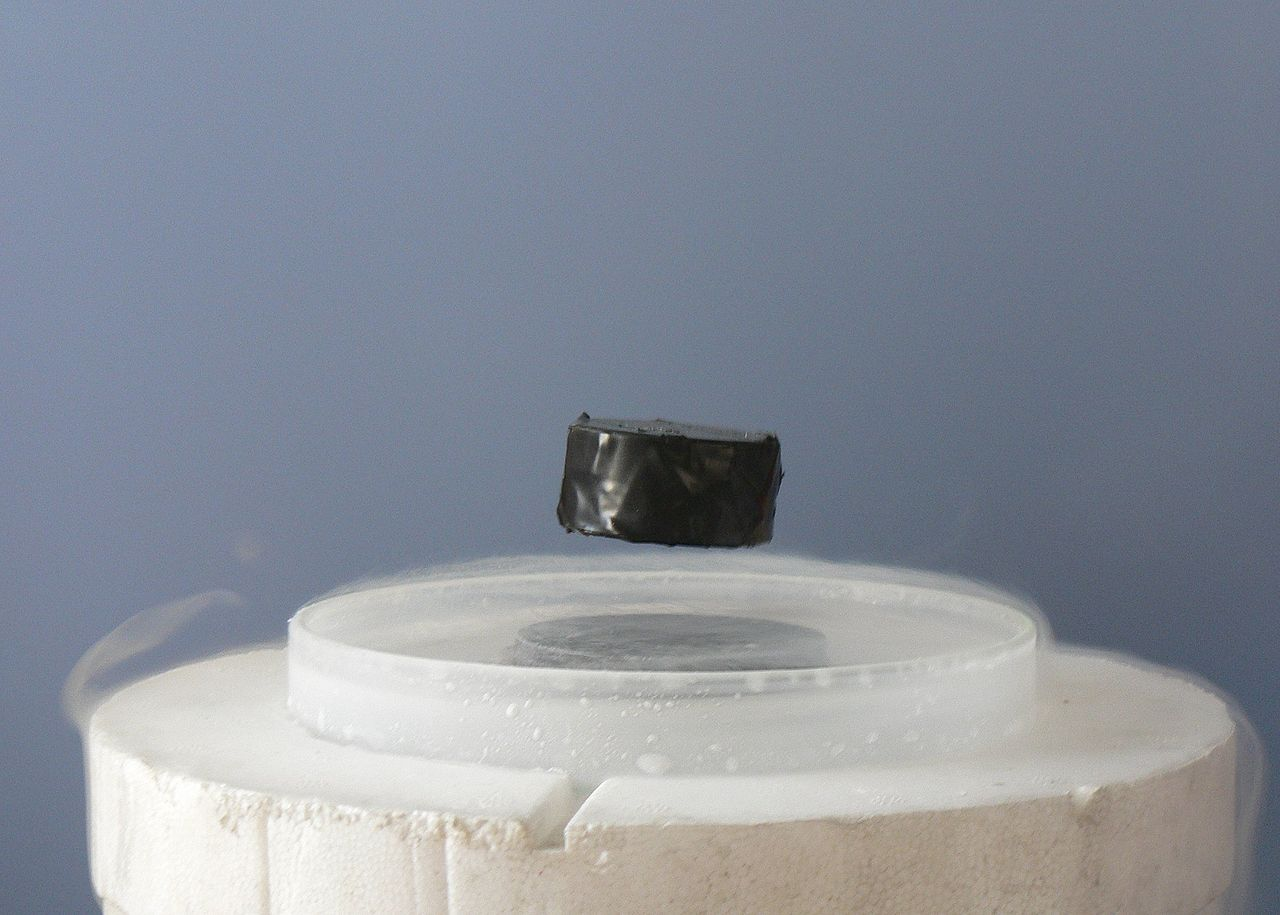
\includegraphics[scale = 0.3]{levitation.jpg}
    \caption{A superconductor levitating over a magnet (Scientific American)}
    \label{fig:my_label}
\end{figure}

Taking the curl of the supercurrent equation and using the Maxwell Eqn $\nabla \mathrm{x} \mathbf{B} = \mu_0 \mathbf{J_s}$ we can find the second London equation:
$$\nabla^2 \mathbf{B} = \frac{1}{\lambda_L^2} \mathbf{B}$$
where $\lambda_L$ is the London penetration depth. This equation describes the Meissner effect: the B field must decay exponentially as you travel into the surface of a superconducting material. This means superconducting materials will resist not just changes in B fields but the B fields themselves.\par 

\subsection{Flux quantization}

Flux quantization is an important effect in superconducting rings. If you apply a B field to a superconducting ring and cool it to below the superconducting temperature for that material, the B field will be forced out of the material by the Meissner effect. Some of the flux will end up trapped in the center of the ring, shown below. \par

\begin{figure}
    \centering
    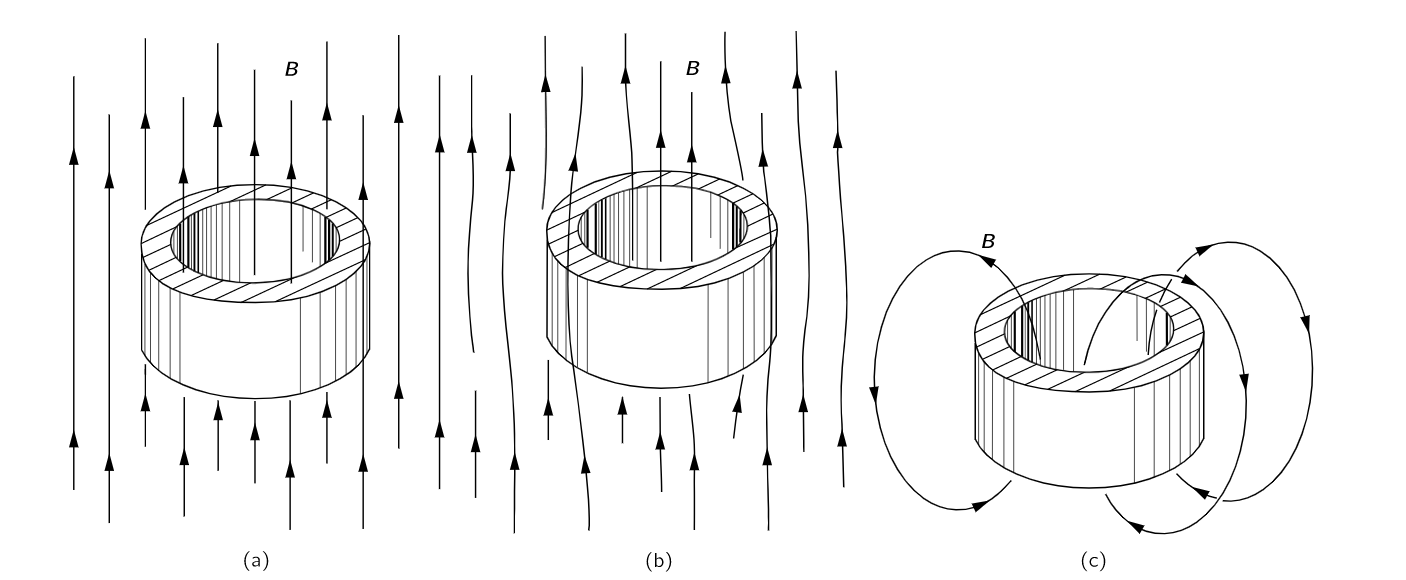
\includegraphics[scale = 0.6]{fluxQuant.PNG}
    \caption{Flux trapping in a superconductor. (a) the ring is in the normal state. (b) the superconducting state. (c) after the external field is removed (Feynman Lectures Vol. 3)}
    \label{fig:my_label}
\end{figure}

Using the equation above for current density in a superconductor and stokes theorem to convert from $\mathbf{A}$ to $\mathbf{B}$, we can derive that around any closed loop,
$$\oint_C (\Lambda \mathbf{J_s}) \cdot dl + \int_S \mathbf{B} \cdot ds = \frac{\hbar}{q^*} \oint_C \nabla \theta \cdot dl$$
The right hand side of this expression should come out to zero because it's the closed line integral of a gradient, but $\theta(\mathbf{r},t)$ is multi-valued because adding a multiple of $2 \pi$ to the phase doesn't change the wave function. The only condition is that the wave function itself has to be continuous. Therefore the integral on the right comes out to $2 \pi n$ and we get: 
$$\oint_C (\Lambda \mathbf{J_s}) \cdot dl + \int_S \mathbf{B} \cdot ds = n\Phi_0 $$
where $\Phi_0$ is the flux quantum and equals $\frac{h}{q^*}$. The left hand side of this equation is the total flux in the loop, both from any external B field present and from the current in the loop. Therefore, the equation states that the total flux in a superconducting loop must be a multiple of the flux quantum. The current in the ring will update so that the trapped flux is one of the acceptable values. 
Flux quantization is a visible effect of the quantum nature of superconductors. The figure below gives a good visualization of how the macroscopic wave function in a superconducting ring forms standing waves, just like the wave function of an electron in an atom.

\begin{figure}[!ht]
    \centering
    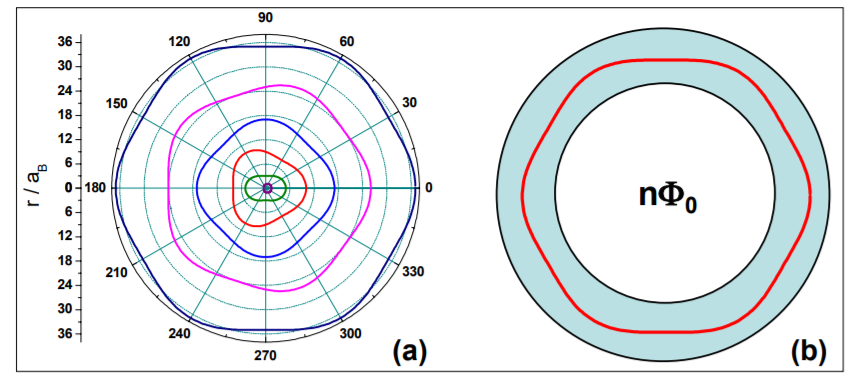
\includegraphics[scale = 0.7]{standingWaves.PNG}
    \caption{(a) standing waves of an electron in an atom, leading to quantized energies. (b) standing waves of the macroscopic wavefunction, leading to quantized flux.}
    \label{fig:my_label}
\end{figure}
\subsection{Quantum Tunneling}
In classical mechanics, we can imagine an object passing through a potential barrier. The object requires an initial kinetic energy greater than or equal to the barrier in order to pass through. If its initial energy is less than the threshold energy, it has zero probability of overcoming the barrier. However, this intuition is dismantled in the quantum regime. 


\begin{figure}[!ht]
    \centering
    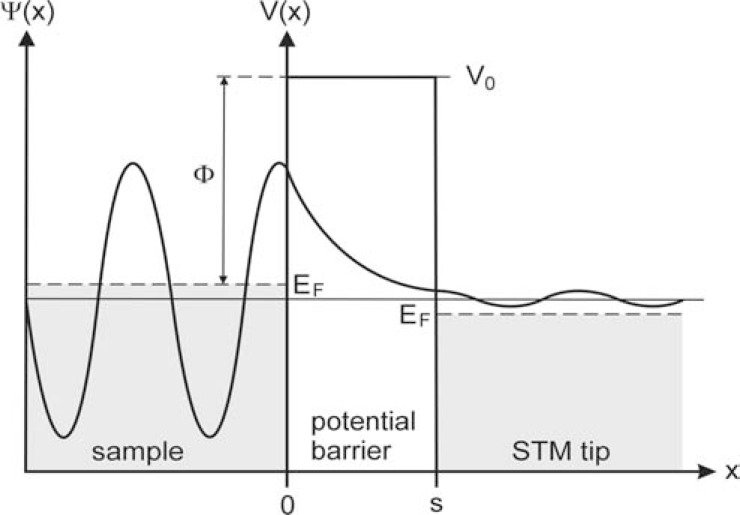
\includegraphics[scale = 3.0]{tunneling.png}
    \caption{Quantum tunneling effect, with Φ has the barrier height, Ef as Fermi Energy, and s has barrier width}
    \label{fig:my_label}
\end{figure}

Quantum tunneling describes the process in which an electron can pass through a voltage barrier despite having lower kinetic energy. Since it exhibits wave-like properties, the electron has a small probability of tunneling through the barrier. The kinetic energy of the electron experiences an exponential decay within the barrier meaning the chance of tunneling dramatically increases as the barrier shortens. 


\subsection{Josephson Effect}
The Josephson effect is of huge importance in quantum computing as most types of qubits rely on it to work. In a Normal Metal / Insulator / Normal Metal junction (NIN junction) electrons have a reasonable probability of tunneling through the insulating barrier if it's thin enough. The probability for a single electron is on the order of $10^{-4}$. Therefore there is a tunneling current associated with the random movement of electrons across the barrier. When the normal metal electrodes are replaced by superconducting metal, it is called an SIS junction, or a Josephson Junction (JJ), shown below. \par 

\begin{figure}[!ht]
    \centering
    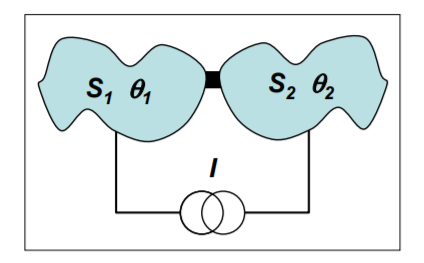
\includegraphics{junction.PNG}
    \caption{A Josephson Junction: the two superconductors S1 and S2 are weakly coupled}
    \label{fig:my_label}
\end{figure}


There is no tunneling current in a JJ. This is because only single electrons are known to tunnel across barriers and not Cooper pairs. Once the voltage between the superconducting electrodes is raised above a certain voltage $\frac{2\Delta}{e}$, called the energy gap voltage, the Cooper pairs are broken up and there is a tunneling current. But below this point the tunneling current is (ideally) 0. \par 
However, there is another current that results from the $\nabla \theta$ term (the phase gradient) in the supercurrent equation. Across small dimensions, this can be simplified into a phase difference $\varphi$. Then there is a supercurrent that results from the weak coupling of the superconductors. This is the Josephson Effect. The supercurrent is proportional to $\sin{\varphi}$ since the wave functions of the superconductors are periodic with the phase. The coupling of the superconductors is analogous to the coupling of electron wave functions in chemically bonded atoms. The effects of these properties will be discussed in the next section on Josephson junctions. 

\subsection{Types of Superconductors}

\pagebreak 
\section{Josephson Junctions}
\subsection{Basic Equations}
As stated in the last section, the 2 superconducting regions in a Josephson Junction are weakly coupled. Assume $\psi_1$ and $\psi_2$ are the amplitudes in the superconductors S1 and S2, there is no external magnetic field, and the junction is connected in series with a battery providing a voltage V (and therefore a potential energy difference qV). Then, the joint Schrodinger equations are: 
$$i\hbar \frac{d\psi_1}{dt} = \frac{qV}{2}\psi_1 + K\psi_2$$
$$i\hbar \frac{d\psi_2}{dt} = -\frac{qV}{2}\psi_2 + K\psi_1$$
Where K is the coupling coefficient that expresses how coupled the two superconductors are. Since $\psi_1$ and $\psi_2$ are the macroscopic wave functions in superconductors, their squared amplitude is the charge density, so we can write $(\psi_1, \psi_2)$ = $\sqrt{(\rho_1, \rho_2)}e^{i(\phi_1, \phi_2)}$. The supercurrent density between S1 and S2 can then be found easily because by definition, $\frac{d\rho_1}{dt} = -\frac{d\rho_2}{dt} = J$. By plugging the wave functions into the above equations we can derive the following relationship between current density and phase: 
$$J = J_0\sin\varphi$$
Where $\varphi = \phi_1 - \phi_2$. The sinusoidal relationship is expected because the wave functions themselves are periodic with the phase.
We can also derive a relationship between the voltage and the phase: 
$$\frac{d\varphi}{dt} = \frac{qV}{\hbar} = \frac{2\pi}{\Phi_0}V$$
Therefore the voltage across the junction is proportional to the time derivative of $\varphi$. 

\subsubsection{Lumped Model}
In reality the line integral $\int_C \mathbf{E} \cdot dl$ is not necessarily constant across all paths $C$ in the area of the junction, so writing V in the above equations assumes the junction area is relatively small. Another assumption that can be made is that $\mathbf{J}$ is relatively constant across the area of the junction. To be exact, the current across a surface $A$ is calculated by $I = \int_A \mathbf{J} \cdot dA$. But with the above assumption we can turn the current density - phase relationship into a current-phase relationship: 
$$I = I_c \sin \varphi$$
Where $I_c$ is called the critical current (it marks the transition between the superconductive and resistive regimes of the junction). This assumption is called the lumped model and allows much easier calculations and circuit modeling of the junction.

\subsubsection{Equivalent Inductance}
A JJ with a voltage applied to it has an inductance. This inductance can be calculated using $V = L\frac{dI}{dt}$ since both I and V are now known as functions of $\varphi$:
$$L_J = \frac{\Phi_0}{2\pi I_c \cos{\varphi}}$$
This inductance is clearly not constant. In a typical linear inductor, a constant voltage will result in a linearly increasing or decreasing current. In a JJ, the current will be sinusoidal instead.

\subsubsection{Josephson Coupling Energy and Washboard Potential}
A linear inductor stores energy in a magnetic field, and this energy depends entirely on its inductance. Likewise, the inductance of a Josephson junction implies that there is energy being stored somewhere. This seems counter-intuitive because unlike other passive elements (e.g. a resistor), there is clearly no power required to sustain a current (the junction is in the superconducting state so $V = 0$, and $P = IV$). However it does take some energy to change the current as this results in a finite $\frac{d\varphi}{dt}$ and therefore a finite $V$. This energy is stored in the coupled wave functions: as we saw in the Schrodinger equations for $\psi_1$ and $\psi_2$ in the superconducting regions, there is energy associated with the K factor. To find the energy put into the junction from when $\varphi(0) = 0$ to when $\varphi(t_0) = \delta$, we can integrate the $I$ times $V$ power and use the Josephson equations: 
\begin{equation}
    \begin{split}
        E_J & = \int_{0}^{t_0} IV dt \\
        & = \int_{0}^{t_0} (I_c \sin{\varphi})(\frac{\Phi_0}{2\pi}\frac{d\varphi}{dt}) \\
        & = \frac{\Phi_0 I_c}{2\pi} \int_{0}^{\delta} \sin \varphi d\varphi \\
        & = \frac{\Phi_0 I_c}{2\pi} (1 - \cos{\delta}) = E_{J0}(1 - \cos{\delta})
    \end{split}
\end{equation}
This energy is called the Josephson coupling energy. With 0 DC current, $E_J$ is the total potential energy of the system. Clearly it is maximized when $\delta = \pi + 2\pi n$ ($\delta$ is the phase difference instead of $\varphi$ in this case). \par
How does $E_{pot}$ change when the junction is biased with a dc current $I$ where $|I| < I_c$? It turns out there is another term added which is proportional to $\varphi$ so the potential becomes: $$E_{pot} = E_{J0}[1 - \cos\varphi - \frac{I}{I_c}\varphi]$$
This results in the potential shown below, called the washboard potential. As the DC current is increased, the potential gets more and more tilted until at $|I| > I_c$, there are no local minima and it becomes unstable. 

\begin{figure}[!ht]
    \centering
    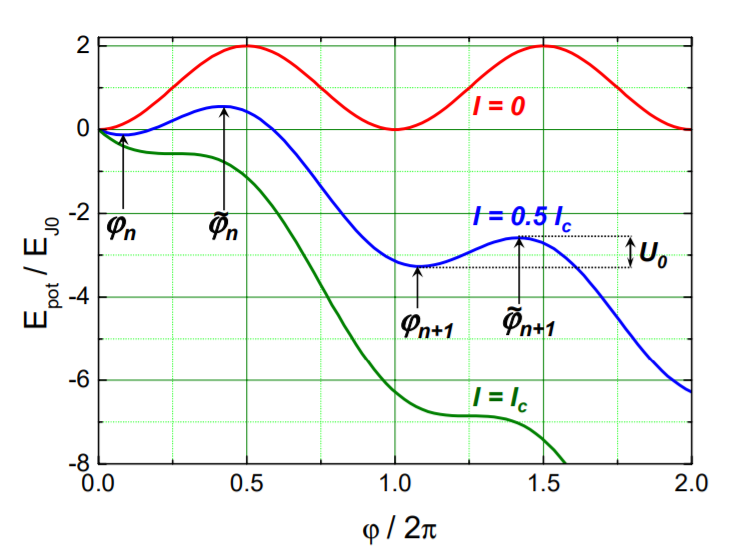
\includegraphics[scale = 0.7]{washboard.PNG}
    \caption{The washboard potential of a Josephson junction. The different curves shown are for different values of I.}
    \label{fig:my_label}
\end{figure}

\subsection{Finite Voltage Circuit Models}
\subsubsection{Equivalent RLC with Noise Current}
There is also a capacitance because a JJ is functionality a capacitor (two conductors separated by a thin insulator). The capacitance is
$$C = \frac{\epsilon A}{d} $$
Where $\epsilon$ is the dielectric constant of the insulator, $A$ is the cross-sectional area of the junction and $d$ is the thickness of the insulator. \par
There is also a resistance. This resistance is based on the current due to quantum tunneling of single electrons across the insulator. As mentioned before, when V is greater than the gap voltage, the Cooper pairs break up and individual electrons tunnel across the barrier. The current is linear with the voltage, with the proportionality constant being $R_N$, the normal resistance. However, there can also be tunneling to a certain extent below the gap voltage if the temperature is high enough. The sub-gap resistance is 
$$ R_{sg} = \frac{n_{tot}}{n(T)}R_n$$
where $n_{tot}$ is the total number of electrons and $n(T)$ is the number of free electrons as a function of temperature. This makes sense as the tunneling current depends on $n(T)$, so the effective resistance should too. Therefore the total resistance is a function of V and T:
\[
    R_N(V,T) = \begin{cases}
    \frac{n_{tot}}{n(T)}R_n, |V| < \frac{2 \Delta(T)}{e}\\
    R_N, |V| > \frac{2 \Delta(T)}{e}
    \end{cases}
\]
So far we have modeled the resistive, capacitive and inductive channels of the junction. These three are added in parallel because the total current is split between the supercurrent, the displacement current and the tunneling current by Kirchhoff's law.\par

\begin{figure}[!ht]
    \centering
    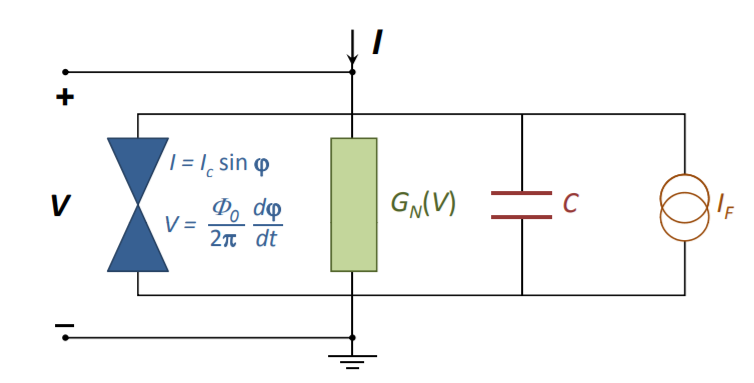
\includegraphics[scale = 0.8]{junctionModel.PNG}
    \caption{The circuit model of the Josephson Junction including a noise current $I_f$. $G_N$ is just the inverse of $R_N$.}
    \label{fig:my_label}
\end{figure}

The last current branch in the circuit model is the noise current. This simulates 3 sources of noise: thermal noise, shot noise and low frequency noise. Thermal noise arises when the voltage is low so that $eV << k_B T$ (The left hand side is the energy imparted to an electron by the applied voltage, and the right-hand side is the energy imparted by heat which is just the temperature times Boltzmann's constant). This type of noise happens even without any applied voltage. It is often modelled as Gaussian white noise. Shot noise is dominant when $eV >> k_B T$. In this case, the noise is caused by the fact that current across the junction is carried by discrete charges, namely electrons. It can be modeled as a Poisson process since each electron moves independently but the average rate (the current) is constant. The 1/f noise is only dominant at frequencies < 1 kHz so it is usually ignored. \par
We can use Kirchhoff's current law to relate the total current to the supercurrent, displacement current, tunneling (or normal) current and noise current: $I = I_s + I_D  + I_N + I_F$. Plugging in the voltage-phase relation and the formulas for the capacitance and resistance, we get 
$$I = I_c \sin\varphi + G_N(V)\frac{\phi_0}{2\pi}\frac{d\varphi}{dt} + C\frac{\phi_0}{2\pi}\frac{d^2\varphi}{dt} + I_F$$

The full model is shown in the figure below.
\subsubsection{Important Parameters}
-McCumber Parameter
-plasma frequency
-time scale of LRC circuit


\subsubsection{RCSJ model}
The above equation is very nonlinear and difficult to solve. The most common simplification of this model is to make the resistance constant. This results in the Resistively and Capacitively Shunted (RCSJ) model. The equation can then be put into the form of the equation describing the motion of a mass in a potential U: 
$$m\frac{d^2x}{dt} + \eta\frac{dx}{dt} + \nabla U = 0$$
Where M is the mass of the particle and $\eta$ is the damping factor. In this case the current acts like a force and the phase difference like the x coordinate. Therefore $M \propto C$, $\eta \propto \frac{1}{R}$ and the potential U is the washboard potential which is obtained from the coupling energy of the junction described earlier. Plugging the potential in and changing the dependent variable from t to $\tau$, the normalized time constant, makes the RCSJ equation:
$$\beta_c \frac{d^2\varphi}{d\tau} + \frac{d\varphi}{d\tau} + \sin\phi - i - i_F(\tau) = 0$$
Where $\beta_c$ is the Stewart-McCumber parameter, and $i$ and $i_F$ are current and noise current respectively divided by the critical current $I_C$. This is analogous to the motion of a pendulum if the noise current is ignored:

\begin{figure}[!ht]
    \centering
    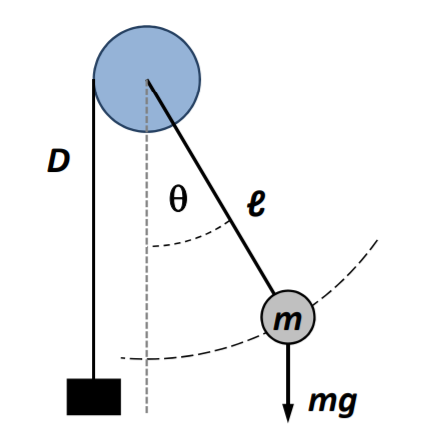
\includegraphics[scale = 0.4]{pendulum.PNG}
    \caption{The motion of a pendulum in gravity with driving torque D. The driving torque is to the pendulum as the total current I is to the JJ.}
    \label{fig:my_label}
\end{figure}

Importantly, the Stewart-McCumber parameter $\beta_c$ determines how damped the system is. A small $\beta_c$ corresponds to a relatively small mass in the pendulum equation, making the system underdamped. A large $\beta_c$ corresponds to a relatively large mass, making the system overdamped. 

\subsubsection{IV Characteristics}
To figure out the IV characteristics for the overdamped and underdamped cases, it helps to consider the washboard potential. The equation of motion in the above section can be interpreted as the motion of a particle of mass m moving along the washboard potential, like so: 

\begin{figure}[!ht]
    \centering
    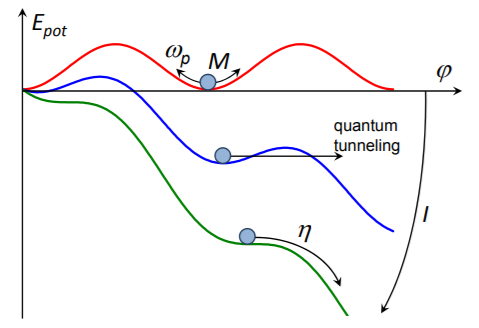
\includegraphics[scale = 0.6]{washboardParticle.PNG}
    \caption{An imaginary particle moving across the surface of $E_{pot}$}
    \label{fig:my_label}
\end{figure}

Since this is a quantum scenario, the particle has a finite probability of tunneling across a potential barrier but that will be ignored now. As discussed before, raising $I$ tilts the potential so that the particle can more easily jump over to the next local minimum. In particular when $I > I_c$, the particle will keep moving in one direction instead of oscillating and the time average of $\frac{d\varphi}{dt}$ (hence the voltage) will be nonzero.  
In the overdamped case, the particle is too massive to gain much momentum even when $I > I_c$. Therefore its momentum stays low and its position is largely determined by the present conditions. However in the underdamped case, the particle is able to gain much more momentum and to slow it back down to the oscillatory state, $I$ has to be lowered to much less than $I_c$. This translates into a hysteretic IV characteristic (meaning the value of I depends not only on V but on the direction, so that it "retains memory") for the underdamped case, as shown below. 

\begin{figure}[!ht]
    \centering
    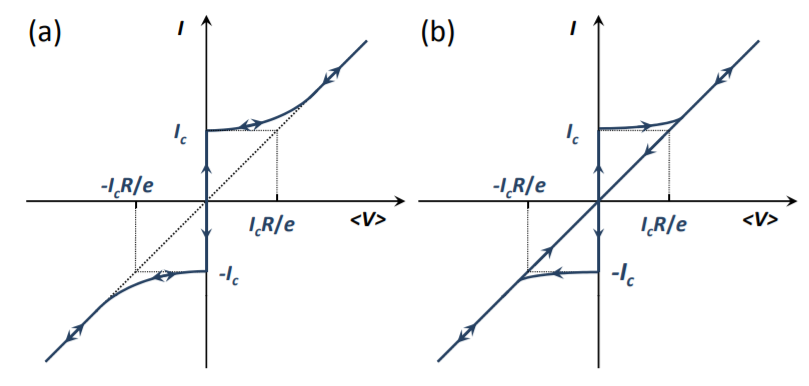
\includegraphics[scale = 0.7]{ivChars.PNG}
    \caption{(a) IVC of overdamped junction which has no hysteresis (b) IVC of underdamped junction with hysteresis. The arrows indicate the direction traveled along the curve.}
    \label{fig:my_label}
\end{figure}

\subsection{Usefulness in Qubits}
Josephson junctions are the only dissipationless, nonlinear devices known and therefore are extremely useful in qubits. Since we know Josephson inductance is give by $L_J = \frac{\Phi_0}{2\pi I_c \cos{\varphi}}$ we can observe the non-linearity in the sec(φ) term. This is significant because we can think of qubits as nonlinear resonators (LC Circuits) formed from the Josephson inductance and junction capacitance. Non-linearity is imperative to isolate the two lowest energy states of the qubit, allowing it to function as such. If the Josephson inductance does not change over the $δ$-wavefunction, the oscillator behaves harmonically and the two qubit states are unusable.  Usable states are created only when the Josephson inductance changes in a non-linear fashion over the the δ-wavefunction, which depends on  $E_j$ and $E_c$.


\subsection{Oxide-Based Josephson Junctions}
\subsubsection{Basic Structure}
The basic structure of an oxide-based Josephson Junction is two superconductors separated by an insulator. 

\subsubsection{Fabrication}
An oxide-based Josephson Junction is fabricated by first depositing a thin film of superconducting metal onto an insulating substrate located in a vacuum chamber. Commonly, the metal used is aluminum and the substrate is silicon. Oxygen is then added to the chamber, forming a layer of aluminum oxide (Al2O3) several nanometers thick. The chamber is then returned to its original vacuum state and a final layer of superconducting metal is added on top. This process is executed at the superconducting critical temperature of aluminum, 1.2 kelvin. 

\subsubsection{Mechanics}
Oxide-based Josephson Junctions rely on quantum tunneling to sustain a current through the junction which is composed of two components. The first is the supercurrent of Cooper Pairs and depends of the Josephson Effects stated above. The second is the quasiparticle current which, at superconducting temperatures, arises when the energy from the bias voltage eV exceeds twice the value of superconducting energy gap Δ. 

The current through a Josephson Junction can be described with the following three effects: the DC Effect, the AC Effect, and the Inverse AC Effect. The DC Effect says that in the absence of any external electromagnetic fields, a DC current will flow through the junction, varying in between -Ic and Ic, where Ic is the critical current or the maximum current that can pass through the material while sustaining the superconducting state. The AC Effect states that, with an applied voltage, the Josephson phase varies linearly and current varies sinusoidally with amplitude Ic and frequency dependent on the voltage. Thus, a Josephson Junction can act as a voltage to frequency converter. The Inverse AC Effect is the inverse of the this, meaning the Josephson Junction can act as a perfect frequency to voltage converter. 



\subsection{Semiconductor Josephson Junctions}

As shown by Simmons \cite{simmons1963generalized} one can generalize the tunneling effect between two separated electrodes to find a tunneling current density, J with units Amps per unit area. Considering a rectangular potential barrier at low applied voltage, V $\sim$ 0:

\begin{equation}
    J = \left[\frac{3}{2s} (2m_e \phi )^{1/2}\right](e/h)^2 V \times \exp{[-(4 \pi s/h)(2 m_e \phi_0)^{1/2}]}
\end{equation}

Where $s$ is the barrier length, $m_e$ is the electron mass, $\phi$ is the phase difference, $e$ is electron charge, $h$ is plank's constant, $\phi_0$ is zero-voltage mean barrier height. Ignoring terms outside of the exponential we can see that $J$ scales like $\exp{[- C s \phi_0 ^{1/2}]}$, where $C = 4 \pi (2m_e)^{1/2}/h$. The fact that semiconductors have lower $\phi_0$ compared to insulators and for the same current density $J$, the size of the barrier $s$ can be increased. This is the most important theoretical takeaway for semiconducting JJ's, they can be manufactured with larger barriers which makes the JJ's easier to produce and more reproducible -- meaning less sensitive to small changes in barrier size.



Nondegeneratively doped crystalline barriers

Degeneratively doped barriers

amorphous

Polycrystalline

 Single Crystal
 
 



\pagebreak
\section{SQUID}

A SQUID, also known as a Superconducting Quantum Interference Device, is an instrument that compiles all the aforementioned physical effects and phenomenons in order to act as a very precise and accurate magnetometer. It is been made into implementations that are capable of measuring magnetic fields on the order of \(10^{-17}\) Teslas. Because of this extreme precision and sensitivity, it has been shown to calculate minuscule fields ranging from animal cardiac activity to brain activity. The Figure below shows examples of some magnetic field strengths of different objects which can be measured with a SQUID.

\begin{figure}[!h]
    \centering
    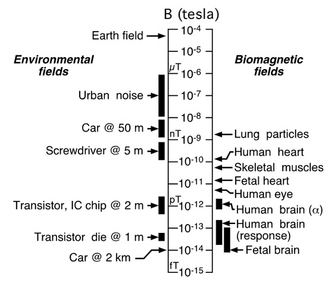
\includegraphics[scale = 0.5]{BFields.jpg}
    \caption{Environmental and Biological field Strengths}
\end{figure}

Depending on the application of the SQUID, they can be manufactured from a multitude of materials. Mainly, they can be made from Type I or Type II superconductors, which differ based on their chemical composition. Type I superconductors are those which are made from pure metals whereas Type II superconductors are those which are made from alloys of metals. The type of superconductor has an effect on the operation of the SQUID namely because of the difference of the Meissner Effect in the two. The Figure below helps to describe this difference. In short, the Meissner Effect will only take place if the magnetic field that a superconductor is exposed to is not too strong. In a Type I superconductor, there is simply only one critical magnetic field under which the Meissner Effect will occur. On the other hand, Type II superconductors have two critical magnetic fields: one which will cause the material to go into what is known as a mixed state in where properties of both superconductors and normal conductors are present, and one which will cause the material to go into the Meissner State in where the Meissner Effect has been noticed. Another factor to take into consideration is that Type I superconductors are capable of having a maximum current density that is approximately ten times larger than that of Type II superconductors. Furthermore, SQUIDs can be manufactured from

\begin{figure}[!h]
    \centering
    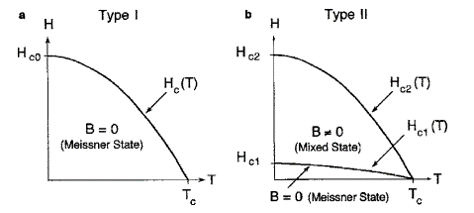
\includegraphics[scale = 0.7]{Meissner.png}
    \caption{Critical Magnetic Fields of Type I and II Superconductors}
\end{figure}

\noindent
High Temperature or Low Temperature Superconductors. As the name implies, these differ based on at what critical temperature the material will go into the superconducting state in where zero resistivity (R=0) has been observed. While these two forms of categorization may appear mutually exclusive, they are not. In fact, all High Temperature Superconductors are Type II superconductors. As mentioned previously, the material used simply depends on the application of the instrument, in some circumstances it may be more appropriate to use a High Temperature Superconductors because the environment simply does not allow for nearly absolute zero cooling conditions. Overall however, SQUIDs that are made from Low Temperature superconductors tend to be more precise and sensitive as a result of the less ambient energy (which we also know as temperature) which has an effect on noise. This precision and sensitivity of course comes at a cost since maintaining these such low temperatures is far less convenient and without a doubt more expensive.

Also depending on the application of the SQUID, they can be designed in two main architectures: the RF SQUID, and the DC SQUID. The RF SQUID stands for the Radio Frequency SQUID and the DC SQUID stands for the Direct Current SQUID. The two differ in operation and construction but in general have the same purpose. The Figure below helps to visualize the difference in construction. In short, the RF SQUID is made with a loop of superconducting material with one Josephson Junction and the DC SQUID is made with two Josephson Junctions in parallel. Aside from

\begin{figure}[!h]
    \centering
    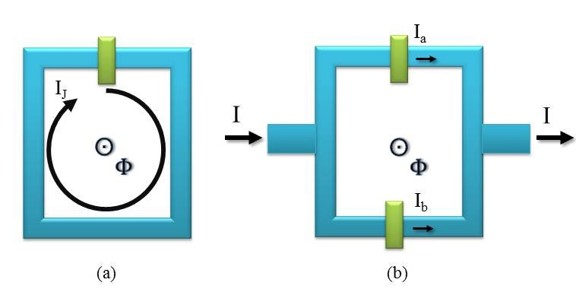
\includegraphics[scale = 0.7]{RFDC.jpg}
    \caption{(a) The RF SQUID and (b) The DC SQUID}
\end{figure}

\noindent
the difference in construction, what gives these two architectures their names are the properties of the applied bias current. The RF SQUID is biased with a current, by an inductively coupled input coil, that oscillates at the radio frequency (so somewhere on the order of \(10^6\) Hertz) and thus relies on the AC Josephson Effect. An important side note: while an RF current is technically an Alternating Current (AC), it oscillates many orders of magnitudes faster and for that reason has interesting physical properties which will be discussed shortly. The DC SQUID is directly biased with a unidirectional current which is equivalent to two times the critical current, the maximum current, of the Josephson Junction (since currents in parallel add). 

Both architectures pose strikingly similar output properties that differ in few ways. For both, the output voltage that is detected is periodically proportional to the input magnetic flux (which is proportional to the magnetic field). And for both, the period of this oscillation is the single flux quantum. The difference of the output properties lies in the shape of the periodic relationship: for RF SQUIDs a saw-tooth relationship exists, and for DC SQUIDs a sinusoidal relationship exists. This can be demonstrated from experimental results in the Figure below. 

\begin{figure}[!h]
    \centering
    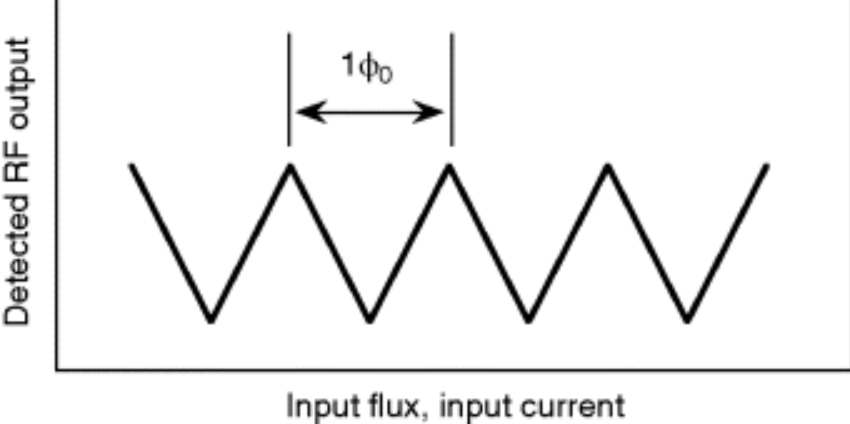
\includegraphics[width = .4\linewidth]{RF.PNG}
    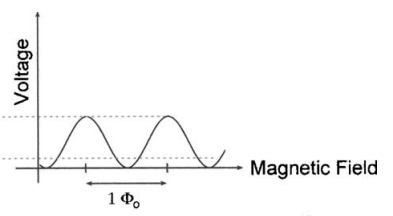
\includegraphics[width = .4\linewidth]{DC.PNG}
    \caption{RF SQUID Output (on the left) and DC SQUID Output (on the right)}
\end{figure}

In terms of high level conceptual understanding, the two architectures function according to very similar principles. When the SQUID is exposed to a magnetic field, the inside of the loop of either architecture will obtain some calculable magnetic flux. The Meissner Effect will then take place, and a current flowing in the opposite direction of the normally induced current (like Lenz's Law) will form on the surface of the SQUID in order to expel the magnetic field lines from penetrating the inside of the superconducting material. This change in current is then calculated by some means, depending on the architecture, in order to determine the strength of the magnetic field which the SQUID was exposed to. For the RF SQUID, an LC circuit is inductively coupled to it and changes in voltages across it are measured as the output. For the DC SQUID, the voltage directly across the parallel Josephson Junctions are measured since the induced current will either flow clockwise or counterclockwise, in effect causing current to flow opposite than the bias current in on of the Josephson Junctions. 

In order to help better understand the physics and output properties of this device, it makes sense to derive the relationship between magnetic flux and current. This is more easily done for a DC SQUID so that is how it will be done here. Using the standard equations of a Josephson Junction which were stated in an earlier section, we can start by coming up with a basic equation for the current through this device without the magnetic flux. While this step is not critical for the derivation, it will resemble the final result and help to get an idea of why the magnetic flux and current relationship exists. This simple parallel circuit can be visualized in the Figure below. 

\begin{figure}[!h]
    \centering
    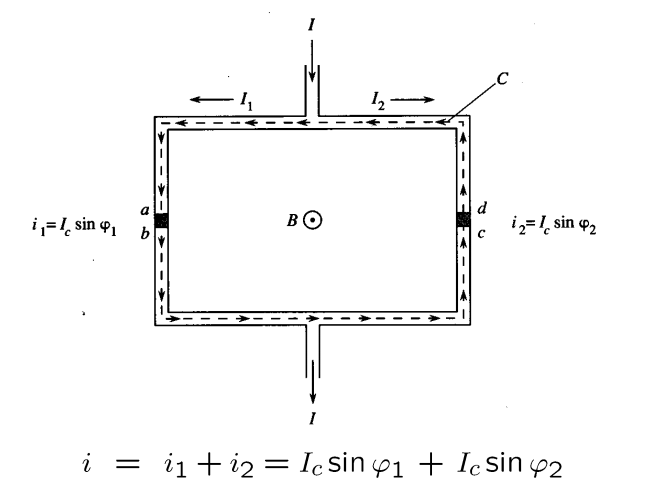
\includegraphics[width = .6\linewidth]{NoFlux.PNG}
    \caption{Independent Current through DC SQUID}
\end{figure}

This relation is simple but in order to derive the relation we desire, we must start by looking at the phase difference from one end of the instrument to the other. This can be done in two ways, one way for each Josephson Junction, as shown below where \(\delta_{a}\) and \(\delta_{b}\) represent the phase differences along their respective junction.

\begin{figure}[!h]
    \centering
    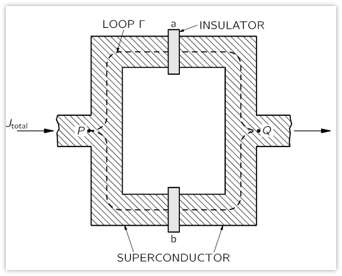
\includegraphics[width = .3\linewidth]{Loop.png}
\end{figure}

$$\Delta Phase_{P\rightarrow Q} = \delta_{a} + \frac{2q_{e}}{\hbar} \int_{upper} \boldsymbol A \cdot d\boldsymbol s$$
$$\Delta Phase_{P\rightarrow Q} = \delta_{b} + \frac{2q_{e}}{\hbar} \int_{lower} \boldsymbol A \cdot d\boldsymbol s$$

Now since these two equations are equal since they both represent the same big picture phase difference, the two can be set equal to each other. With that done, we can then perform some algebra to get an equation for the difference of the phase differences along the two junctions. When doing this algebra, we can combine the line integrals of the vector potential field (\boldsymbol A) into a single line integral of \boldsymbol A over the arbitrary loop \(\Gamma\) through the device. While it may seem that the two line integrals would subtract to zero, in fact one must be initially negated since in the two equations for the phase difference, the vector potential field is assumed to be parallel to the bias current when over the loop \(\Gamma\) they should be antiparallel. This leaves us with the following equation. 

$$\delta_{b} - \delta_{a} = \frac{2q_{e}}{\hbar} \oint_{\Gamma} \boldsymbol A \cdot d\boldsymbol s$$

Where, 

$$\oint \boldsymbol A \cdot d\boldsymbol s = \Phi $$

So,

$$\delta_{b} - \delta_{a} = \frac{2q_{e}}{\hbar} \Phi $$

Using this, we can break up our difference equation into two individual equations that represents how each phase difference changes as a flux is applied, where \(\delta_{0}\) represents the initial phase difference along the respective Josephson Junction.

$$\delta_{a} = \delta_{0} - \frac{q_{e}}{\hbar}\Phi$$
$$\delta_{b} = \delta_{0} + \frac{q_{e}}{\hbar}\Phi$$

With these equations for how the phase difference changes with the applied flux, we be plug this back into the current equation that we obtained before we started our derivation, leaving us with the equation below.

$$I_{total} = I_{C}(\sin{(\delta_{0} - \frac{q_{e}}{\hbar}\Phi)} + \sin{(\delta_{0} + \frac{q_{e}}{\hbar}\Phi)})$$

With this equation, the sinusoidal relationship between the magnetic flux and the current is more visible. Furthermore, we can see a maximum current of 

$$I_{max} = 2I_{0}|\cos{\frac{q_e}{\hbar}\Phi}|.$$

Which occurs with a periodicity of  

$$\Phi = n \frac{\pi\hbar}{q_{e}}.$$

Where the single flux quantum is

$$\Phi_{0} = \frac{\pi\hbar}{q_{e}} \approx 2 \times 10^{-7} gauss \cdot cm^{2} .$$

Below is an image provided from experimental results of the operation of a DC SQUID. The images provided above simply were a more zoomed in portion of this graph. The SQUID is not very capable of measuring stronger magnetic fields because of the effect that the Meissner Effect will cease to take place once the magnetic field strength exceeds the critical magnetic field.

\begin{figure}[!h]
    \centering
    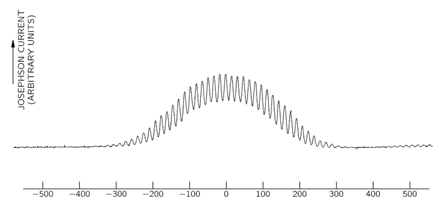
\includegraphics[width = .6\linewidth]{Result.png}
    \caption{Experimental Results for DC SQUID}
\end{figure}

\pagebreak

Now with a clearer conceptual and mathematical understanding, there are some nuances to go over. The main one being that the equation that was just derived is in some sense a simplified equation. This is because of the fact that the magnetic flux going through the loop is not only the effect of the external magnetic field but also from a self induced magnetic flux which comes from the fact that a SQUID inevitably has its own inductance. This is because any loop of conducting material is in some sense an inductor. As a result of this fact, the magnetic flux going through the loop can be more accurately described by 

$$\Phi_{total} = \Phi_{ext} + L_{SQUID}I_{cir}.$$

Where 

$$I_{cir} = (i_{1} - i_{2})/2.$$

Engineers and physicists attempt to minimize the effect of this self induced magnetic flux by decreasing the physical size of the loop since this decreases its inductance however this inevitably has some inverse effects. While the inductance of the SQUID is decreased, so is the SQUID's sensitivity. In an attempt to combat this, manufacturers will more often than not use what is called a flux transformer. A flux transformer is an instrument that is used to trap more magnetic flux than what the SQUID can and then transfer it into a smaller range so that it can have an effect on the SQUID. Images of different variations of flux transformers can be seen below. Not only does this instrument allow for the reduction of the self induced magnetic flux, but it allows the SQUID to have a wider range of application as the Figure implies. 

\begin{figure}[!h]
    \centering
    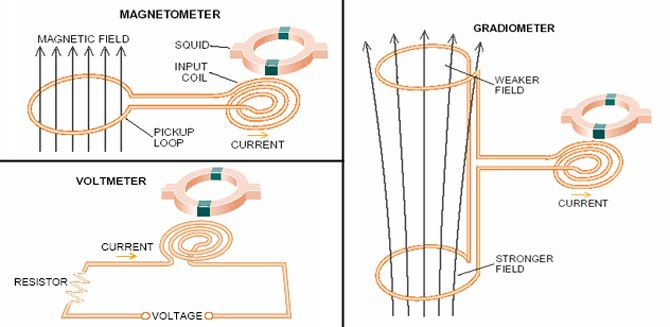
\includegraphics[width = .7\linewidth]{fluxtransformer.jpg}
    \caption{Variations of Flux Transformers}
\end{figure}

RF SQUIDs and DC SQUIDs have their own realms in which they perform best in. In general however, the DC SQUID tends to be the one that is used for more precise and sensitive measurement due to the fact that the RF SQUID is bias with a Radio Frequency current. Since the current oscillates so fast, lots of energy radiates into the surrounding environment as radio waves. Like working with High Temperature Superconductors, the energy that is in the surrounding environment leads to hysterical effects which can prevent the device from working quantum mechanically. For this reason, when very precise and sensitive measurements are required, the Low Temperature DC SQUID tends to be the instrument of choice (and in fact was the first SQUID created).

As mentioned in the first paragraph of this section, SQUIDs have a variety of applications such as measuring biological processes in living animals. However, this is not the only place they are used. Just to name of few, SQUIDs have been used in Magnetic Resonance Imagine (MRI) machines, military devices, and (as you may have guessed) quantum computers! More specifically on the last one, there have been implementations in which SQUIDs have been used for flux and even phase qubits. Being first invented in the 1960s, the SQUID is still known as one of the most sensitive instruments for measuring we have today.

\pagebreak
\section{SFQ electronics}
\subsubsection{Types of Logic Devices}
Josephson Junctions (JJ's) have utility for use in classical computing as well as quantum computing. For classical computing, there are 2 ways to represent logic with the state of a JJ: latching and non-latching logic. Latching logic relies on the hysteresis effect of underdamped JJ's to represent the "on" state with the voltage across the junction. The drawback to this is that there is a delay in switching back to the "off" state that limits the frequencies of these devices to just above 1 GHz. Therefore, non-latching logic has been the focus for decades due to its shorter gate delay and smaller power dissipation than latching logic. Non-latching logic so far has been implemented up to speeds of several hundred GHz. 
\subsubsection{RSFQ Devices}
The main technology used in non-latching logic is Rapid Single Flux Quantum (RSFQ). In these devices "on" and "off" states are encoded by the presence or absence of pulses, rather than the voltage across the JJ. When a JJ is biased slightly above $I_c$, instead of a sinusoidal voltage waveform the voltage takes the form of pulses (think about the particle speeding up and slowing down abruptly as it falls down the washboard potential). Using the voltage-phase relation and the fact that the phase changes by $2\pi$ over one pulse, the exact area of these pulses can be easily derived to be the flux quantum:
$$\int V dt = \int \frac{\hbar}{2e} d\phi = \Phi_0$$

\pagebreak
\section{Resonators}
\pagebreak
\section{Qubit and multi-Q systems}
\pagebreak
\section {Qubits in a system: Qiskit}



\nocite{*}
\bibliography{ref}

\end{document}
